%%
%% This is file `sample-sigconf.tex',
%% generated with the docstrip utility.
%%
%% The original source files were:
%%
%% samples.dtx  (with options: `sigconf')
%% 
%% IMPORTANT NOTICE:
%% 
%% For the copyright see the source file.
%% 
%% Any modified versions of this file must be renamed
%% with new filenames distinct from sample-sigconf.tex.
%% 
%% For distribution of the original source see the terms
%% for copying and modification in the file samples.dtx.
%% 
%% This generated file may be distributed as long as the
%% original source files, as listed above, are part of the
%% same distribution. (The sources need not necessarily be
%% in the same archive or directory.)
%%
%%
%% Commands for TeXCount
%TC:macro \cite [option:text,text]
%TC:macro \citep [option:text,text]
%TC:macro \citet [option:text,text]
%TC:envir table 0 1
%TC:envir table* 0 1
%TC:envir tabular [ignore] word
%TC:envir displaymath 0 word
%TC:envir math 0 word
%TC:envir comment 0 0
%%
%%
%% The first command in your LaTeX source must be the \documentclass
%% command.
%%
%% For submission and review of your manuscript please change the
%% command to \documentclass[manuscript, screen, review]{acmart}.
%%
%% When submitting camera ready or to TAPS, please change the command
%% to \documentclass[sigconf]{acmart} or whichever template is required
%% for your publication.
%%
%%
\documentclass[sigconf]{acmart}

%%
%% \BibTeX command to typeset BibTeX logo in the docs
\AtBeginDocument{%
  \providecommand\BibTeX{{%
    Bib\TeX}}}

%% Rights management information.  This information is sent to you
%% when you complete the rights form.  These commands have SAMPLE
%% values in them; it is your responsibility as an author to replace
%% the commands and values with those provided to you when you
%% complete the rights form.
\copyrightyear{2023}
\acmYear{2023}
\setcopyright{acmlicensed}
\acmConference[ICAIL 2023]{Nineteenth International Conference on Artificial Intelligence and Law}{June 19--23, 2023}{Braga, Portugal}
\acmBooktitle{Nineteenth International Conference on Artificial Intelligence and Law (ICAIL 2023), June 19--23, 2023, Braga, Portugal}
\acmPrice{15.00}
\acmDOI{10.1145/3594536.3595173}
\acmISBN{979-8-4007-0197-9/23/06}

%%
%% Submission ID.
%% Use this when submitting an article to a sponsored event. You'll
%% receive a unique submission ID from the organizers
%% of the event, and this ID should be used as the parameter to this command.
%%\acmSubmissionID{123-A56-BU3}

%%
%% For managing citations, it is recommended to use bibliography
%% files in BibTeX format.
%%
%% You can then either use BibTeX with the ACM-Reference-Format style,
%% or BibLaTeX with the acmnumeric or acmauthoryear sytles, that include
%% support for advanced citation of software artefact from the
%% biblatex-software package, also separately available on CTAN.
%%
%% Look at the sample-*-biblatex.tex files for templates showcasing
%% the biblatex styles.
%%

%%
%% The majority of ACM publications use numbered citations and
%% references.  The command \citestyle{authoryear} switches to the
%% "author year" style.
%%
%% If you are preparing content for an event
%% sponsored by ACM SIGGRAPH, you must use the "author year" style of
%% citations and references.
%% Uncommenting
%% the next command will enable that style.
%%\citestyle{acmauthoryear}

\usepackage{framed}


%%
%% end of the preamble, start of the body of the document source.
\begin{document}

%%
%% The "title" command has an optional parameter,
%% allowing the author to define a "short title" to be used in page headers.
\title{A Dataset of German Legal Reference Annotations}

%%
%% The "author" command and its associated commands are used to define
%% the authors and their affiliations.
\author{Harshil Darji}
\orcid{0000-0002-8055-1376}
\affiliation{%
  \institution{University of Passau}
  \country{Germany}
  \postcode{94032}
}
\email{Harshil.Darji@uni-passau.de}

\author{Jelena Mitrović}
\orcid{0000-0003-3220-8749}
\affiliation{%
  \institution{University of Passau}
  \country{Germany}
  \postcode{94032}
}
\affiliation{%
  \institution{Institute for AI R\&D of Serbia}
  %\city{Novi Sad}
  \country{Serbia}
  \postcode{21000}
}
\email{Jelena.Mitrovic@uni-passau.de}

\author{Michael Granitzer}
\orcid{0000-0003-3566-5507}
\affiliation{%
  \institution{University of Passau}
  \country{Germany}
  \postcode{94032}
}
\email{Michael.Granitzer@uni-passau.de}


%%
%% By default, the full list of authors will be used in the page
%% headers. Often, this list is too long, and will overlap
%% other information printed in the page headers. This command allows
%% the author to define a more concise list
%% of authors' names for this purpose.
\renewcommand{\shortauthors}{Darji et al.}

%%
%% The abstract is a short summary of the work to be presented in the
%% article.
\begin{abstract}
The field of legal Natural Language Processing faces a lot of challenges due to the unavailability of properly structured datasets. One such instance is the need for a dataset that not only separates different parts of legal references, such as an article or paragraph number but also provides information about what a particular legal reference dictates. Having access to such a dataset can provide easy access to researchers working on experiments such as context similarity between law texts and legal cases that refer to a particular law. In this paper, we present a dataset of 2944 legal references in German law that are manually annotated by law experts. This dataset has 21 properties for each law reference in the dataset, such as \textit{Buch}, \textit{Teil}, \textit{Titel}, \textit{Untertitel}, etc. It also provides the complete text of each law reference in the dataset, along with specific paragraph text mentioned in the law reference. Furthermore, using this dataset together with Open Legal Data, we perform a law reference prediction task to compare the performance between predicting full law reference and only the base law reference.
\end{abstract}

%%
%% The code below is generated by the tool at http://dl.acm.org/ccs.cfm.
%% Please copy and paste the code instead of the example below.
%%
\begin{CCSXML}
<ccs2012>
   <concept>
       <concept_id>10010147.10010178.10010179.10003352</concept_id>
       <concept_desc>Computing methodologies~Information extraction</concept_desc>
       <concept_significance>500</concept_significance>
       </concept>
   <concept>
       <concept_id>10010147.10010257.10010293.10010294</concept_id>
       <concept_desc>Computing methodologies~Neural networks</concept_desc>
       <concept_significance>300</concept_significance>
       </concept>
 </ccs2012>
\end{CCSXML}

\ccsdesc[500]{Computing methodologies~Information extraction}
\ccsdesc[300]{Computing methodologies~Neural networks}

%%
%% Keywords. The author(s) should pick words that accurately describe
%% the work being presented. Separate the keywords with commas.
\keywords{Legal Language Processing, NLP, Sentence Transformers, Open Legal Data, Law References, Law Reference Annotations}

%\received{20 February 200}
%\received[revised]{12 March 2009}
%\received[accepted]{5 June 2009}

%%
%% This command processes the author and affiliation and title
%% information and builds the first part of the formatted document.
\maketitle

\section{Introduction}
\label{sec:introduction}

In the legal field, the amount of data is growing more and more every day, while digitization faces the same challenges as every other field. Manually processing and analyzing this much data is truly a monotonous and time-consuming task. For this reason, legal NLP and Legal Tech aim at applying state-of-the-art computer science techniques to improve and speed up this process. The use and significance of Artificial Intelligence in the legal domain for reasoning with cases and argumentation are expressed in \cite{governatori2022thirty}. Studies mentioned in this paper show that the use of computing methodologies for reasoning with legal cases goes as far back as 1987 \cite{10.1145/41735.41743}. However, one of the bottlenecks here is the lack of properly structured datasets on which new models or approaches can safely be trained and published. Lack of access to such properly structured datasets in the legal domain acts as a barrier for researchers working in Legal Tech \cite{bradford2019competition,xiao2018cail2018}.

Datasets in the German legal domain that are currently available mainly focus on providing the entirety of legal cases, e.g. Open Legal Data\footnote{\url{https://de.openlegaldata.io/}}, or named entities in those legal cases such as the Legal Entity Recognition dataset \cite{leitner2020dataset}. However, there are certain tasks such as comparing contextual similarities between a legal case and the law text this case refers to, or analyzing the importance of law in reference to other laws. For such tasks, it is necessary to have a dataset of legal references that not only provides researchers with full texts for each legal reference mentioned in a given legal case but also text from a specific paragraph, if required.

The legal references in the dataset we are presenting here are obtained from the Open Legal Dataset using a German BERT model \cite{chan2020german} trained on the Legal Entity Recognition dataset \cite{leitner2020dataset}. These legal references are then manually annotated, including a link to their online version. We conducted experiments on law reference prediction tasks using Open Legal Data. Our goal was to predict both full law references and base law references from this dataset.

\section{Related work}

There are very few open and available legal datasets for German law, one of which is Open Legal Data, published by Ostendorff et al. \cite{ostendorff2020towards} in 2020. This dataset contains metadata for more than 250,000 German laws and court decisions. The primary source for this dataset are courts and government data, as they have the highest level of reliability. Secondary sources are scrapping data directly from trusted websites such as Gesetze im Internet\footnote{\url{https://www.gesetze-im-internet.de/}} and Rechtsprechung im Internet\footnote{\url{https://www.rechtsprechung-im-internet.de/}}, and Linked Open Data.

Another important dataset was published by Leitner et al. \cite{leitner2020dataset} in 2019. This dataset was generated for Named Entity Recognition in German federal court decisions. It contains approximately 67,000 sentences and 54,000 manually annotated entities. These entities are characterized into 7 coarse-grained classes: \textit{Person, Location, Organization, Legal norm, Case-by-case regulation, Court decision, and Legal literature}. These are further sub-characterized into 19 fine-grained classes: \textit{person, judge, lawyer, country, city, street, landscape, organization, company, institution, court, brand, law, ordinance, European legal norm, regulation, contract, court decision, and legal literature}. The dataset is publicly available in the CoNNL-2002 format \cite{sang2003introduction} on GitHub\footnote{\url{https://github.com/elenanereiss/Legal-Entity-Recognition/tree/master/data}}.

Furthermore, Urchs et al.\cite{inproceedings} published another important dataset in 2021. It is available in two parts, one consists of a total of 32,748 decisions from 131 German courts, while the second part consists of 200 randomly chosen judgments. The judgments in the second part of the dataset are annotated with the conclusion, definition, and subsumption annotations.

In \cite{urchs2020towards}, Urchs et al. also identified and addressed the lack of availability of German legal corpora that follows the \textit{Urteilsstil} writing style for German judgments. As stated by the authors, this writing style ``\textit{begins with the conclusion and proceeds with the reasoning}". To create the corpus, the authors crawled over 30,000 court decisions from \url{www.gesetze-bayern.de}. Out of these court decisions, 11,477 are judgments. The authors then proceeded with 200 randomly selected judgments for manual annotations and published them as one part of the dataset. The second part consists of 30,000 court decisions with \textit{Name of the court, Type of the court decision, Date of the court decision, Reference number, Title of the court decision, Norm chains, Place of reference} metadata.

Other than these publicly available datasets, there are a few cost-based databases such as juris\footnote{\url{https://www.juris.de/}}, beck-online\footnote{\url{https://beck-online.beck.de/}}, LexisNexis\footnote{\url{https://www.lexisnexis.de/}}, and Wolters Kluwer Online\footnote{\url{https://www.wolterskluwer-online.de/}}. All these datasets contain a large number of case records, federal statutes, commentaries, and more.

To the best of our knowledge, there is no publicly available dataset for the German legal domain that provides researchers with full or partial texts of law references for a legal case.

\section{Dataset}
\label{sec:dataset}

In this section, we explain the process of gathering data from Open Legal Data, extracting law references from this data using Transformers \cite{vaswani2017attention}, and finally, annotating these law references.

\subsection{Pre-processing Open Legal Data}
In order to create a dataset of law reference annotations, we first need a list of law references to annotate. For this purpose, we gathered the case records from the Open Legal Data, preprocessed them, and created a new dataset of clean Open Legal Data, which is currently publicly available at zenodo\footnote{\url{https://zenodo.org/record/6631931\#.ZDfYE-xBz0o}}. This dataset is approximately 1.1 GB in size and contains 43337 rows and the following 12 features.

\begin{table}[h]
\centering
\caption{Features in the clean Open Legal Data dataset with statistics.}
\label{tab:dataset-old}
\begin{tabular}{|l|c|}
\hline
\textbf{Features} & \textbf{Total} \\
\hline
id & 43337 \\
slug & 43337 \\
ecli & 10831 \\
date & 43337 \\
court & 43337 \\
jurisdiction & 43337 \\
level\_of\_appeal & 43337 \\
type & 43337 \\
tenor & 36282 \\
tatbestand & 24243 \\
gründe & 27144 \\
entscheidungsgründe & 24038 \\
\hline
\end{tabular}
\end{table}
The next step is to extract law references from this dataset. Various ways to accomplish this task include pattern matching as law references usually start with the article sign ("§") \cite{DBLP:conf/ic3k/MilzGM21}. However, we decided to take a slightly different approach using a transformer\cite{vaswani2017attention} model.

\subsection{German BERT for Legal NER}
To extract law references from pre-processed Open Legal Data, we use a German BERT\footnote{\url{https://www.deepset.ai/german-bert}} model fine-tuned on the Legal Entity Recognition dataset mentioned in related works with a micro-F1 score of 99.49\cite{icaart23}. This fine-tuned German BERT is available on HuggingFace\footnote{\url{https://huggingface.co/harshildarji/gbert-legal-ner}}. We then used this fine-tuned model on the  \textit{tenor}, \textit{tatbestand}, \textit{gründe}, and \textit{entscheidungsgründe} parts of the clean Open Legal Data to extract law references.

Three legal experts, who have already passed their first state examinations in law, manually annotated 21 labels for the law references. To ensure that the annotation task was correctly set up, they performed a test annotation task on 523 law references. The level of agreement between the three annotators was then measured by Fleiss' kappa score, which has been calculated to be 0.87, indicating a strong inter-annotator agreement. Afterward, the annotators worked independently on annotating the remaining law references using all the physical and digital legal resources necessary for the tasks. These 21 annotation labels are as follows:\\

\begin{framed}
{\textit{Gesetzbuch/Norm, Buch , Teil, Abschnitt, Titel, Untertitel, Kapitel, Artikel, Absatz, Buchstabe, Unterabsatz, Satz, Nummer, Buchstabe , Online Link Gesetzbuch, Online Link Exakt, Alternative Schreibweise 1, Alternative Schreibweise 2, law\_title, full\_text, absatz\_text}}
\end{framed}

Here, \textit{Gesetzbuch/Norm} refers to the standard written description of a specific law, \textit{Online Link Gesetzbuch} refers to the link to the base of the law, while \textit{Online Link Exakt} refers to the link to the specific article of the law. \textit{Alternative Schreibweise 1} and \textit{Alternative Schreibweise 2} show the normalized variant to write a law reference. 

For example, given a law reference, \textbf{\textit{Art. 1 Abs. 1 GG}}\footnote{\url{https://www.gesetze-im-internet.de/gg/art_1.html}}, \textit{Gesetzbuch/Norm} is \textbf{\textit{Grundgesetz}}, the base of the law is \textbf{\textit{GG}}, and the specific article is \textbf{\textit{Art. 1}}. \textit{Alternative Schreibweise 1} and \textit{Alternative Schreibweise 2} is \textbf{\textit{Art. 1 (1) GG}} and \textbf{\textit{Art. 1 I GG }}.

\subsection{Gathering corresponding law texts}
Next, we use the links available in \textit{Online Link Exakt} to get the \textit{law\_title}, \textit{full\_text}, and \textit{absatz\_text}. However, we were not able to get these details for all the law references due to various reasons such as some laws not being in German or specified \textit{Absatz} not being available in the linked text.

For the above example, the \textit{law\_title} is \textbf{\textit{Grundgesetz für die Bundesrepublik Deutschland Art 1}}, the \textit{full\_text} is\\

\begin{framed}
{\textit{(1) Die Würde des Menschen ist unantastbar. Sie zu achten und zu schützen ist Verpflichtung aller staatlichen Gewalt.\\
(2) Das Deutsche Volk bekennt sich darum zu unverletzlichen und unveräußerlichen Menschenrechten als Grundlage jeder menschlichen Gemeinschaft, ...},}
\end{framed}

and the \textit{absatz\_text} is\\

\begin{framed}
{\textit{(1) Die Würde des Menschen ist unantastbar. Sie zu achten und zu schützen ist Verpflichtung aller staatlichen Gewalt}.}
\end{framed}

Also, some law references in the dataset simply refer to the base article. Therefore, there are also law references for which many features have absent values, as shown in Table \ref{tab:dataset-nan}.

\begin{table}[h]
\centering
\caption{Number of absent values for each feature in our dataset, with the English translation of each feature.}
\label{tab:dataset-nan}
\begin{tabular}{|l|l|c|}
\hline
\textbf{Features} & \textbf{English} & \textbf{Absent}\\
\hline
Referenz & Reference & 0 \\ 
Gesetzbuch /Norm & Code/Norm & 0 \\ 
Buch & Book & 2264 \\
Teil & Part & 1943 \\
Abschnitt & Section & 674 \\
Titel & Title & 2484 \\
Untertitel & Subtitle & 2872 \\
Kapitel & Chapter & 2294 \\
Artikel & Article & 0 \\
Absatz & Paragraph & 971 \\
Buchstabe & Letter & 2933 \\
Unterabsatz & Subparagraph & 2926 \\
Satz & Sentence & 2129 \\
Nummer & Number & 2543 \\
Buchstabe & Letter & 2928 \\
Online Link Gesetzbuch & Online link law book & 0 \\
Online Link Exakt & Online link Exact & 0 \\
Alternative Schreibweise 1 & Alternate spelling 1 & 11 \\
Alternative Schreibweise 2 & Alternate spelling 2 & 11 \\
law\_title & Law title & 0 \\
full\_text & Full text & 1 \\
absatz\_text & Paragraph text & 973 \\
\hline
\end{tabular}
\end{table}

Figure \ref{fig:Gesetzbuch} shows the total number of occurrences of law reference for the top-10 Gesetzbuch /Norm.

\begin{figure}
    \centering
    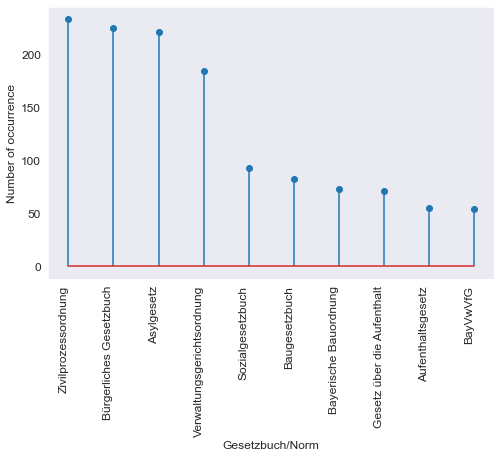
\includegraphics[width=1.0\linewidth]{latex/gesetzbuch.png}
   \caption{Number of law reference for top-10 Gesetzbuch/Norm}
   \label{fig:Gesetzbuch}
\end{figure}

As we can see in Figure \ref{fig:Gesetzbuch}, the most used \textit{Gesetzbuch /Norm} is \textit{Zivilprozessordnung}, which translates to Code of Civil Procedure. This law is mainly used to regulate actions in civil courts, where one civilian of a country can sue another to resolve a dispute between them.

Figure \ref{fig:Gesetzbuch-art} shows the total number of occurrences of law reference for the top-10 Gesetzbuch/Norm and article combination. The plot shows that the most used law reference is \textit{Gesetz über die Aufenthalt, die Erwerbstätigkeit und die Integration von Ausländern im Bundesgebiet 1}, which translates to \textit{Act on the Residence, Employment and Integration of Foreigners in Federal Territory 1}. This law is used to govern the residence and employment of nationals from a different country of origin. This high occurrence can be explained by a higher number of case records in the clean Open Legal Data from 2015 and 2016. 2015 was a year of migration crisis across Europe due to several civil wars in Lybia, Syria, and Iraq. Germany accepted a total of 1,091,894 and 321,361 refugees in 2015 and 2016, respectively\footnote{\url{https://www.statista.com/statistics/911484/number-newly-registered-refugees-germany/}}.

\begin{figure}
    \centering
    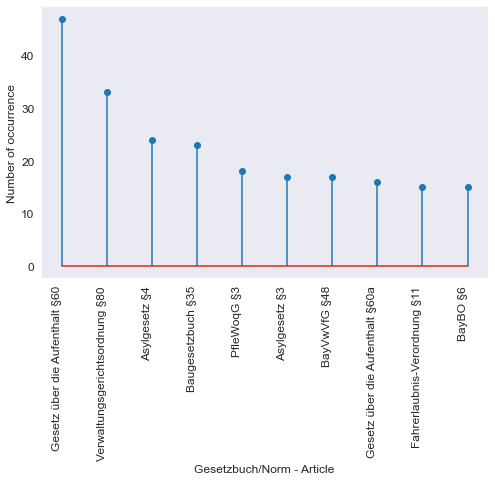
\includegraphics[width=1.0\linewidth]{latex/gesetzbuch-art.png}
   \caption{Number of law reference for top-10 Gesetzbuch/Norm-Article}
   \label{fig:Gesetzbuch-art}
\end{figure}

\section{Experiments}
\label{sec:experiment}

In this section, we show how this dataset can be used in practice. In our previous research \cite{darji_mitrović_granitzer}, we identified that case texts that refer to the same law are closely grouped in an embedding space. Therefore, it is safe to say that we can use these embeddings to predict law references, given case text. We also fine-tune the German BERT model to predict law references, given law texts. Here, we perform prediction based on the base law reference (e.g. \textit{§ 97 ZPO.}) and the full law reference (e.g. \textit{§ 97 Abs. 1 ZPO.}).

\subsection{Predicting base law references}

Here, we experiment with predicting only the base law referred to in the case text, while ignoring the \textit{Absatz} or \textit{Satz} part of the law reference. For example, given two law references, \textit{§ 86b Abs. 1 SGG} and \textit{§ 86b Abs. 2 Satz 2 SGG}, we train the model to only predict only the base law, which in this case is \textit{§ 86b SGG}.

In our dataset, over 50\% of data refers to the top 20 base law references, which is approximately 7\% of unique base law references available. Therefore, we train our model to predict these top 20 base law references, making this essentially a 20-class classification problem.

In order to make sure the underlying German BERT model is trained on an equal amount of data for each class label, we perform a stratified train-test split of the dataset. Figure \ref{fig:base_plot} shows the performance of fine-tuning the German BERT model.

\begin{figure}[h]
	\centering
	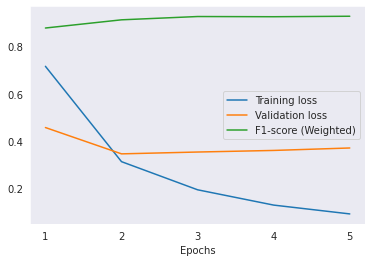
\includegraphics[width=0.9\linewidth]{latex/plot.png}
	\caption{Performance of fine-tuning the German BERT model to predict base law references. The fine-tuned model provides a consistent performance of 0.9 weighted F1-score just after the second epoch.}
	\label{fig:base_plot}
\end{figure}

The bar plot in Figure \ref{fig:base_bar_plot} shows the performance for individual base law references.

\begin{figure}[h]
	\centering
	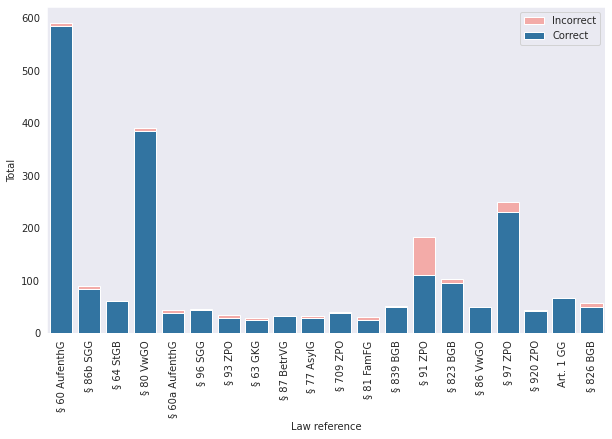
\includegraphics[width=1\linewidth]{latex/base_correct.png}
	\caption{Bar plot visualizing the number of correctly predicted base law references compared to incorrect predictions.}
	\label{fig:base_bar_plot}
\end{figure}

\subsection{Predicting full law references}

Here, we fine-tune the German BERT model to predict full law references as they appear in the case text. Similar to predicting the base law references, we treat this task as a 20-class classification problem. This is because, similar to base law references, over 50\% of the dataset refers to the top 20 law references available in our dataset. Here as well, we perform a label-wise stratified train-test split over the dataset.

Figure \ref{fig:full_plot} shows the performance of fine-tuning the German BERT model, while the bar plot in Figure \ref{fig:full_bar_plot} shows the performance for individual full law references.

\begin{figure}[h]
	\centering
	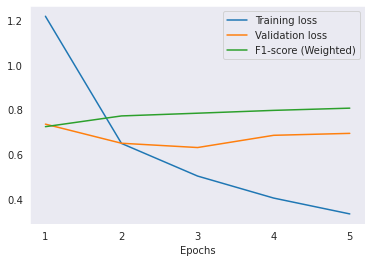
\includegraphics[width=0.9\linewidth]{latex/full_plot.png}
	\caption{Performance of fine-tuning the German BERT model to predict full law references. After five epochs, the fine-tuned model provides an approximate performance of 0.8 weighted F1-score.}
	\label{fig:full_plot}
\end{figure}

\begin{figure}[h]
	\centering
	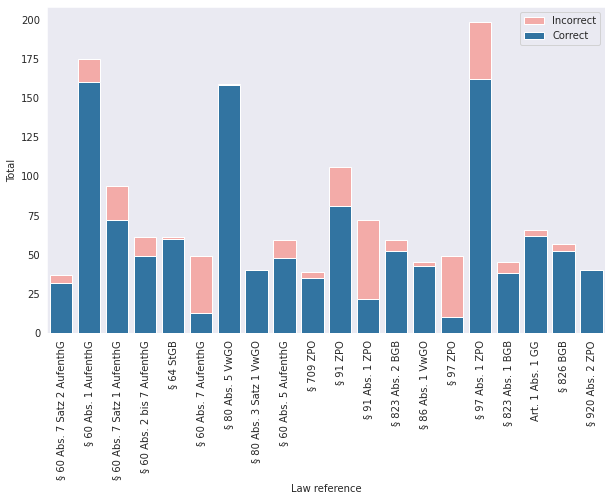
\includegraphics[width=1\linewidth]{latex/full_bar_plot.png}
	\caption{Bar plot visualizing the number of correctly predicted full law references compared to incorrect predictions.}
	\label{fig:full_bar_plot}
\end{figure}

Table \ref{tab:val-perform} shows the validation performance for predicting the base law references and full law references.

\begin{table}[h]
\centering
\caption{Accuracy and weighted performances for the base and full law reference prediction.}
\label{tab:val-perform}
\begin{tabular}{|l|c|c|}
\hline
\textbf{Metrics} & \textbf{Base law reference} & \textbf{Full law reference} \\
\hline
Accuracy & 0.92853 & 0.81336 \\
Weighted-Precision & 0.92994 & 0.80539 \\
Weighted-Recall & 0.92853 & 0.81336 \\
Weighted-F1 & 0.92707 & 0.80565 \\
\hline
\end{tabular}
\end{table}

\section{Conclusion}
\label{sec:conclusion}

In this paper, we present a dataset of annotations for legal references done by legal experts. This dataset will enable NLP researchers working with legal data to avoid crawling and scrapping data from different sites to gather information about law references.

One of the ways to use this dataset is shown in section 4, where we perform a law reference prediction task, using full law reference and base law reference. Results from this experiment indicate that the task of predicting base law references gives a much better performance than the task of predicting full law references.

The overlapping behavior of semantically similar case text with similar base law references suggests that we can use sentence embeddings to perform the link prediction tasks. This is one of the future tasks that can be performed using this dataset - to identify instances of case texts very similar to queried case text with a specific law reference.

\section{Acknowledgments}

\begin{figure}[h]

\includegraphics[width=2.5cm]{latex/BMBF.jpeg}
\end{figure} 

The project on which this report is based was funded by the German Federal Ministry of Education and Research (BMBF) under the funding code 01|S20049, and also partially by the project DEEP WRITE (Grant No. 16DHBKI059). The author is responsible for the content of this publication.

\bibliographystyle{ACM-Reference-Format}
\bibliography{sample-base}

\end{document}
\endinput
%%
%% End of file `sample-sigconf.tex'.
